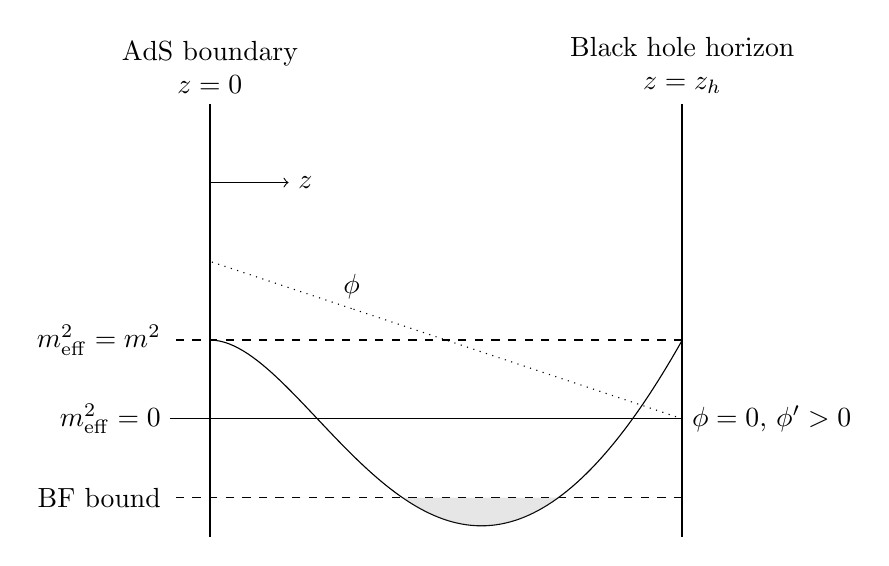
\begin{tikzpicture}
    \draw[->] (0,3) -- (1,3) node[right] {$z$};
    \draw[-,thick] (0,-1.5) -- (0,4) node[above,align=center] {AdS boundary\\$z=0$};
    \draw[-,thick] (6,-1.5) -- (6,4) node[above,align=center] {Black hole horizon\\$z=z_h$};
    \draw[-] (6,0) -- (-0.5,0) node[left] {$m_{\mathrm{eff}}^2=0$};
    \draw[-] (6,1) -- (-0.5,1)[dashed] node[left] {$m_{\mathrm{eff}}^2=m^2$};
    \draw[-] (6,-1) -- (-0.5,-1)[dashed] node[left] {BF bound};
    \draw[dotted] plot[domain=1:0.3,samples=50] (\x*6,{2*(1-\x)})node[above] {$\phi$};
    \draw[dotted] plot[domain=0.3:0,samples=50] (\x*6,{2*(1-\x)});
    \draw[-] (6,0) node[right] {$\phi=0$, $\phi^\prime>0$};
    \draw[solid] plot[domain=0:1,samples=100] (\x*6,{1-2*\x*\x/(1-\x*\x*\x)*4*(1-\x)*4*(1-\x)});
    \draw [fill=gray,fill opacity=0.2,draw=none] plot[domain=0:1,samples=100] (\x*6,{-1}) -- plot[domain=0:1,samples=100] (\x*6,{min(1-2*\x*\x/(1-\x*\x*\x)*4*(1-\x)*4*(1-\x),-1)});
\end{tikzpicture}